\chapter{Machine Learning}
\label{chp:machine_learning}

Machine learning is a way of using statistics to solve problems either by learning from a data set how what the output should be for an input or by figure out different patterns in the data. This is called supervised and unsupervised learning respectively. It is widely used in spam filtering and search engines.

\section{The Basics}
The basics for machine learning is to use to the computer to create a model from which the computer is able to predict the output or category of an input based on the values of the input. 
Machine learning most often consists of two phases, training and testing. The training phase is where the algorithm learns the model and works out how to categorize the data, and testing is where a new dataset is used to see how accurate the algorithm is. 
In this report supervised and unsupervised learning is used. Supervised learning means the data has a label of which it is meant to be categorized as, and unsupervised use unlabeled data with the assumption that the majority of data is considered normal.

\section{Anomaly Detection}
Anomaly detection, also called outlier detection, is a problem very suited for machine learning. It is a way of identify observations or data which doesn't fit an expected pattern. These observations will be referred to as anomalies or outliers in this report. Illustrated in \fref{fig:anomalyExample} is an example of anomalies in a two-dimensional data set. $N_1$ and $N_2$ is the normal areas where most of the observations are, $o_1$ and $o_2$ are anomalies and $O_3$ is an area with multiple anomalies. 

\begin{figure}
\centering
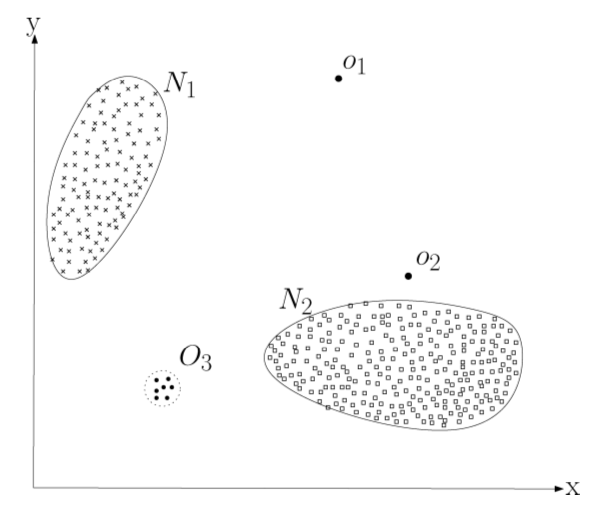
\includegraphics[scale=0.3]{figs/anomaly_example.png}
\label{fig:anomalyExample}
\caption{Example of anomalies in a 2D dataset\citep{chandola2009anomaly}.}
\end{figure}

